\documentclass[12pt,a4paper]{report}
\usepackage{graphicx}
\usepackage{color}
\usepackage{xcolor}
\usepackage{titlesec}
\usepackage{listings}
\usepackage{caption}
\usepackage{appendix}
%\usepackage{minted}
\usepackage{enumitem}
\usepackage{mathtools}
\usepackage{csquotes}
\usepackage{indentfirst}
\usepackage{seqsplit}
\usepackage{float}
\usepackage[colorlinks,allcolors=black]{hyperref} %чтобы ссылки работали 
\usepackage{courier}
\definecolor{light-gray}{gray}{0.95} %цвет фона для кода 

\makeatletter
\renewcommand{\thesection}{%
  \ifnum\c@chapter<1 \@arabic\c@section
  \else \thechapter.\@arabic\c@section
  \fi
}
\renewcommand{\thefigure}{\thesection.\arabic{figure}} %не разобрался с renewcommand выше, написал свою (Б)
\makeatother

\lstset{
    basicstyle=\small,  %or \small or \footnotesize etc.
    breaklines=true, 
    frame=single,
    numbers=left,
    backgroundcolor=\color{light-gray},
}

\usepackage{geometry}
\geometry{
	a4paper,
	left=20mm,
	right=10mm,
	top=10mm,
	bottom=20mm,
}


\titleformat{\chapter}[block]
  {\normalfont\huge\bfseries}{\thechapter.}{1em}{\Huge}
\titlespacing*{\chapter}{0pt}{-19pt}{0pt}

\begin{document}

\begin{titlepage}
	\centering
	{\scshape\LARGE Innopolis University \par}
	\vspace{1cm}
	{\huge\bfseries Secure Systems and Networks\par}
	{\huge\bfseries Research project\par}
	\vspace{2cm}
	\vfill

\begin{minipage}{0.4\textwidth}
\begin{flushleft} \large
\emph{Submitted By:}
\\Vasiliy Podtikhov,
\\Bulat Saifullin,
\\Timur Samigullin
\end{flushleft}
\end{minipage}
~
\begin{minipage}{0.4\textwidth}
\begin{flushright} \large
\emph{Submitted To:}
\\Rasheed Hussain
\\Azat Safin
\\Konstantin Urysov
\\Kirill Saltanov
\end{flushright}
\end{minipage}\\[1cm]

% If you don't want a supervisor, uncomment the two lines below and remove the section above
%\Large \emph{Author:}\\
%John \textsc{Smith}\\[3cm] % Your name

%	supervised by\par
%	Kirill Saltanov
	\vfill
	{\large \today\par}
\end{titlepage}

\tableofcontents  % можно убрать

\begin{abstract}
In modern day social networks become widely used. Practically almost all employers using them. But they can be used to formating public opinion in way not acceptable by company, or by accident share some confidentially information. This often happened because ordinary employee don't unaware of global company goals.

In this work we will try to link a social identity to an IP address by analysis of user traffics. This will help us to establish leakage, find disgruntled employees and change company politics to prevent this situations.
\end{abstract}

\section{Introduction}
Mapping IP address to account on social network is generally believed to be difficult for an individual with no dedicated infrastructure or privileged information. Social networks owners such as Vk.com and Facebook.com have this information, but they always hide it except in the case of a legal decision. But this information may be very handy in big corporations. In average 60\% of employee actively use social networks [1]. And sometime employees post trade secret in social network, usually they use fake name. But if the employee go in  account while he in the corporation's network mapping IP address to account on social network, can help us to find him.

\section{Related Work}
Today we widely used Netflow analysis for security reasons [2][3]. But only recently science works was introduced whom main goal was – determine users action in social networks [4][5]. Unfortunately method who helped us to identify user never was introduced. In this paper we tried to find a solution for this problem.

\section{Research question}
Our research question is: 
\begin{itemize}
	\item{How to map ip addresses to profile in social network by analysing users activity? }
\end{itemize}

To answer this, the following subquestions should be answered:
\begin{itemize}
	\item{Find connection between user traffic and profile changes.}
	\item{What sending data affects changes in profile?}
	\item{How to analysis user's net-flow traffics?}
	\item{How to analysis a profile in social network?}
\end{itemize}


\section{Methodologies}
NetFlow is a feature that was introduced on Cisco routers that provides the ability to collect IP network traffic as it enters or exits an interface. By analyzing the data provided by NetFlow, a network administrator can determine things such as the source and destination of traffic, class of service, and the causes of congestion. A typical flow monitoring setup (using NetFlow) consists of three main components\cite{methodologies1}:
\begin{itemize}
	\item{Flow exporter: aggregates packets into flows and exports flow records towards one or more flow collectors.}
	\item{Flow collector: responsible for reception, storage and pre-processing of flow data received from a flow exporter.}
	\item{Analysis application: analyzes received flow data in the context of intrusion detection or traffic profiling, for example.}
\end{itemize}

We analysed netflow dumps in corporation environment and tried to check if connection was established in period of time and check presence of person in this time period on site. The main purpose is to find correlations between posted time and netflow traffic.


In this work each member of our research group takes responsibility for the most known social networks(vk.com[], instagram.com[], Fecebook.com[]).
\bigbreak
Team members contribution:
\begin{itemize}
	\item{V. Podtikhov - Facebook, Selenium+Phantomjs}
	\item{B. Saifullin - VK, pynfdump}
	\item{T. Samigullin - Instagram, Netflow sample.}
\end{itemize}



%\section{Common things}

% B.tex (for normal text)
\section{VK}
Vk.com is the most popular social network in Russia. Today vk has about 400 millions accounts. 80 millions visitors come to the site every day. 
\subsection{Getting data from vk}
Vk.com provide great api for developers. API interface allows information to be received from the database vk.com with the help of http-requests to the special server. We do not need to know in detail how the base is constructed and from which table and field types it consists of. It is enough that API-request “knows” it. The request syntax and the type of data being returned are strictly determined by the service itself. 
For example, to receive data about the user with the ID number "396547478", we need to make a request of this type:


\begin{lstlisting}
https://api.vk.com/method/users.get?user_ids=396547478&fields=online,last_seen&v=5.60
\end{lstlisting}

Let’s have a look at the individual parts:
\begin{itemize}
	\item{\texttt{api.vk.com/methods} — API server address}
	\item{\texttt{users.get} — name of API VKontakte’s “method”. Methods represent conditional commands that correspond with an operation from the database to receive, record or delete information. For example, users.get is a method to receive information about a user.}
	\item{\texttt{user{\_}ids=396547478{\&}fields=online,last{\_}seen{\&}v=5.60}  – parameter request.}
\end{itemize}
	
In its response, the server returns JSON-object with the requested data (or a message about a mistake if something went wrong). 

The response to our request looks like this:
\begin{lstlisting}
{"response":[{"id":396547478,"first_name":"Ssn","last_name":"Project","online":0,"last_seen":{"time":1480705322,"platform":7}}]}
\end{lstlisting}

Let’s have a close look at fields that is interesting for us:
\begin{itemize}
	\item{\texttt{online} - information whether the user is online.  Returned values: 1 - online, 0 - offline.  If user utilizes a mobile application or site mobile version, it returns \texttt{online{\_}mobile} additional field that includes 1.}  
	\item{\texttt{last{\_}seen}	 - last visit date.  Returns \texttt{last{\_}seen} object with the following fields:
	\begin{itemize}
		\item{\texttt{time} - last visit date (in Unix time).}
		\item{\texttt{platform} - type of the platform that used for the last authorization.}
	\end{itemize}}
\end{itemize}

In this paper we will use only two methods: users.get which returns detailed information on users and wall.get which returns a list of posts on a user wall or community wall.


\subsection{Find ip range of vk}
Vk.com has two ip range 87.240.128.0/18 and 95.213.0.0/18. To figure it out we first ping vk.com, when we take given IP and check information about it by using utility \texttt{whois} it gives us the network mask for this IP. Also we check that vk.com dose not have any another IP by using utility \texttt{dig}, we check that it don't return any another IP addresses.


\subsection{Experimental results}
For the experiments we created test profile https://vk.com/id396547478 and fill wall with some text posts in different times of days. For netflow collection we will use nfdump\cite{nfdump}, and for real test we will use real netflow traffic from university Innopolis. 
\subsubsection{Matching IP to profile by analyzing wall posts}
Wall post can be different format(music, video, link, repost, photo, text message, etc). The text posts is the popular one and it is very hard for analysis, because it is very similar to personal text message that people send to each other every second in private dialogs. So you can not see difference between them in the netflow traffic. We are lucky if a user posts photo, it has 3 fields that we can analyze: post publish time, photo upload time, photo size. But we will look only at difficult case when all post it is small text message similar to the message that users exchange in dialogs. If we able match IP in this case we will able do it in easier case, because text message posts has only one field for analysis: post publish time. For analyze of user wall post and netflow traffic was written program in python language that take last n post, get timestamp from it and for each timestamp it create list with all unique IP that do request to vk in this second($\pm$1 s.) Then it print IPs that was spotted in each list. In figure \ref{fig:wall} you can see we correlation between matched IP and number of post. 
 
\begin{figure}[H]%\label{wall}   [\ref{wall}]
	\centering
		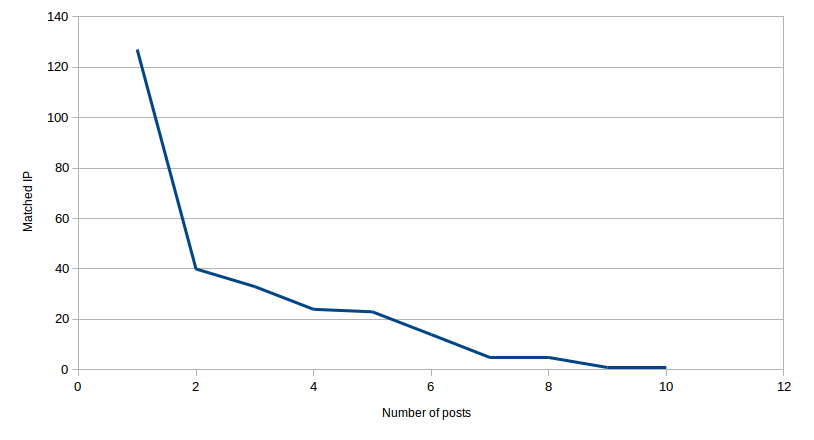
\includegraphics[width=180mm]{images/vk/wall.png}
	\caption{correlation between matched IP and number of post}
	\label{fig:wall}
\end{figure}

\subsubsection{Problems}
The main problem we did not know that the user post posts from the same ip, only that we can know it was or PC or mobile app. 

The second main problem that we have too many active user in the same time. As you can see from figure \ref{fig:users} in peak time we have about 350 unique ip do request to vk server. 

The third problem, it can be less then 9 post with the same IP addresses (from diagram \ref{fig:wall} we saw that we need more then 9 post to match IP). User can do post from different locations, not only in work place and DHCP can change IP too often.

Solutions for this problems will be consider in next section.
\begin{figure}[H]
	\centering
		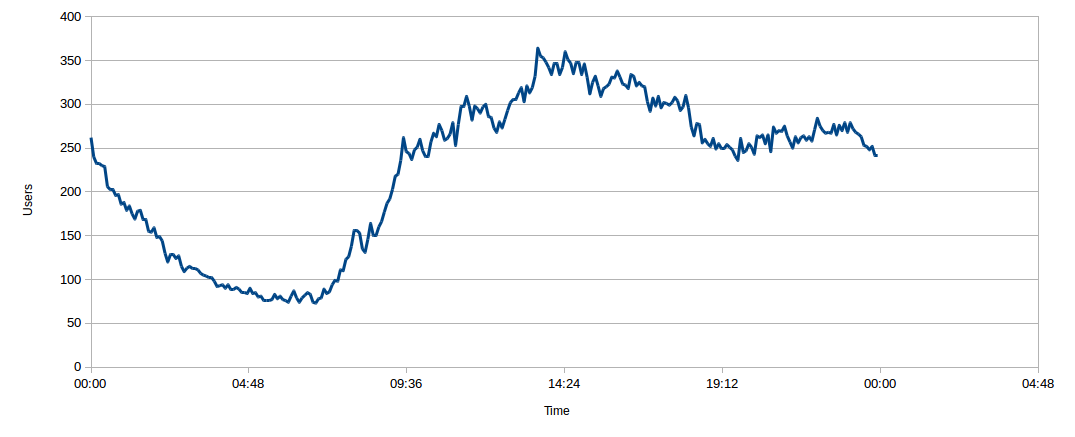
\includegraphics[width=180mm]{images/vk/users.png}
	\caption{Number of vk active users in UI}
	\label{fig:users}
\end{figure}
\subsubsection{Matching IP to profile while user is online}
We can handle all problems that listed above by collecting enough data while user is online. It is highly unlikely that user will post 9 post in his wall per one connections, but he can comment under some post or do post in another wall. But it still hard to collect and  analyze data. We can use social engineering and try to make chat with him, in this case each message can be considered as wall post message(each message has send timestamp like post publish(send) timestamp). But still it can fail if user will not answer. 

After analyze of vk-API by me was found one bug in vk.com (or feature?). In vk page if user is offline in status bar we can see his last seen time, but this field is available from API even when user is online and it update after each activity of user(send message to smb, reload page, do comment or post, open smb page, etc). So we can see that user do something in the site, of curse we don't know what exactly he do, we can just guessing. But now we know what vk server receive some date from user in this exact time.

For exploit this bug we will write two python script, one will check user last seen field and write it in the file each time it change, second program will analyze the file. Because all timestamp will be get in short period it is possible that a lot of another users has connections in this time (they can just watch film in vk) so we will need more timestamp, but now it is not a problem. The correlation between matched IP and number of timestamp you can see in figure \ref{fig:online}. In this figure was consider the case when user is texting with someone. We can see time of each message he send, usually people send 2-3 message per minute and we will get around 50 timestamps in 20 minutes. In this case we need only 42 time stamps to match the IP. 

Program usage:

\texttt{\$ python user{\_}follow{\_}file.py [vk id]}

\texttt{\$ python user{\_}last{\_}seen.py [vk id]}

Output:

\texttt{1 188.130.155.46 	50/50 100\%}

\texttt{2 10.241.1.2    	48/50 96\%}

\texttt{3 10.242.1.90   	47/50 94\%}

\texttt{4 10.90.131.101 	46/50 92\%}


\begin{figure} [H]
	\centering
		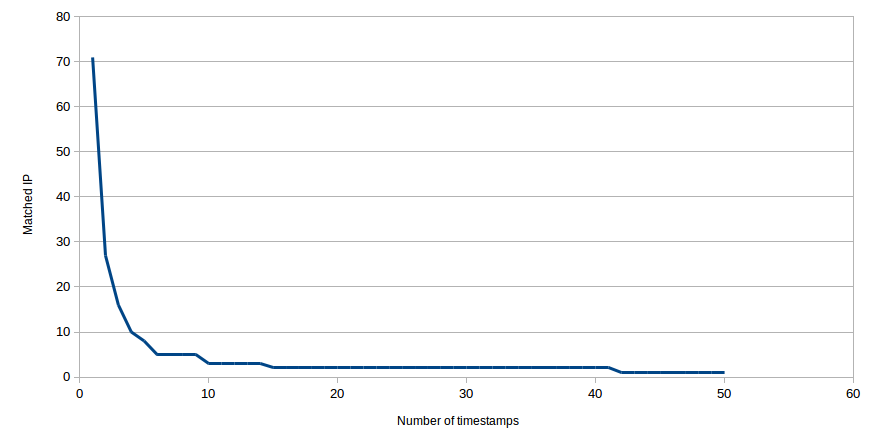
\includegraphics[width=180mm]{images/vk/online.png}
	\caption{The correlation between matched IP and number of timestamp}
	\label{fig:online}
\end{figure}




\section{Instagram}

Instagram is an online mobile photo-sharing, video-sharing, and social networking service that enables its users to take pictures and videos, and share them either publicly or privately on the app, as well as through a variety of other social networking platforms, such as Facebook, Twitter, Tumblr, and Flickr. \cite{instagram1}

\subsection{Getting data from Instagram}

To find correlation between posted time and netflow traffic, we need to get exact time, when user post photo.

Fisrst, all information about post was getting through API functional of Instagram web-site. For this reason third-part application should be registered at instagram development page, and access-token should be got. Request method for getting info about specific post shown bellow:

\begin{lstlisting}
https://api.instagram.com/v1/media/shortcode/BNPjFcrh22_?access_token=3955223166.3a064fe.2562f48363ac48f8b002f713fddeae2e
\end{lstlisting}

With testing accounts everything was fine, but when I tried to access to another real account I have a API error. Instagram API has one speciality: there is a sandbox environment for testing reasons, and for getting data from every page, first, he should be invited to sandbox and he should accept requests from application, even if page open for everybody. I think, application should not ask requests for viewing user's page. 

The way out is to parse raw html page, and get data from it. In source of html page I saw, that there is raw json data.

\begin{figure}[H]
	\centering{
		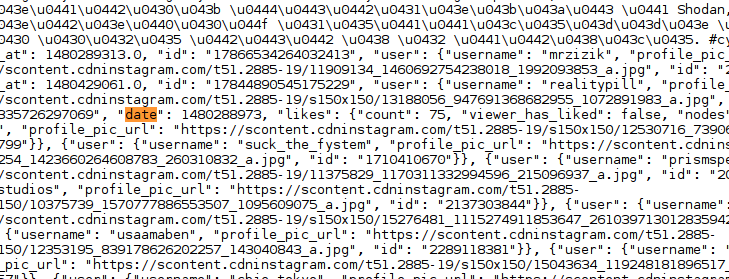
\includegraphics[width=120mm]{images/instagram/1.png}
	}
\end{figure}

It means, that I can simply get all data from specific web page even without any authorization. For parsing I used xpath and re library from python. 

\begin{lstlisting}
script = html.xpath('//script[contains(., "window._sharedData")]/text()')[0]
data = re.search(r"window._sharedData = (.*?);\$", script).group(1)
data = json.loads(data)
\end{lstlisting}

All data was stored in \textbf{data} array.

\subsection{Finding range of instagram ip}

We ask to give us all university netflow traffic for analyzing, it is stored on our computers. The difference of Instagram in comparison with other social network, is that Instagram has very narrow area of usage. In this network users can only add and comment their photos. Every user’s action connected with photos. It means, that instagram need less computer capacity, than other networks. And also Instagram now belong to facebook. The problem was to find exact range of Instagram ip addresses. 

Instagram hasn’t got it’s own autonomous system, but most number of requests send to 31.13.93.72 or 31.13.92.32 or 31.13.93.54. For the first sight we can assume that we should only restrict 31.13.92.0/24 or 31.13.93.0/24. But that is not a solution, because not every address in this network belongs to Instagram.

So, I deсided to find all Instagram ip addresses by myself. I extract all unique destination ip addresses from netflow traffic and get 106 MB file with 6291215 lines. I write a script to revesre-resolve all ip addresses and find Instagram string in it. It was bad idea. Script worked for three days, but process was not finished. And during this I find another solution for this. I decided to use all 31.13.0.0/16 network, and resolve Instagram ip addresses after it.

\subsection{Extracting data from netflow}

In my script I used only raw nfdump. You can see the whole string filter bellow:

\begin{lstlisting}
\$ nfdump -R /var/flows/MYROUTER "dst net 31.13.0.0/16 and port 443" -o csv -t 2016/11/27.22:47:26-2016/11/27.22:47:56 -s record/bytes | head -n -3 | sed '1d'
\end{lstlisting}

The result of such execution:

\begin{lstlisting}
('2016-11-29 15:57:36', '10.240.20.237', '31.13.72.53', '40166', '255667')
('2016-11-29 15:57:22', '10.91.35.114', '31.13.72.8', '57339', '15368')
('2016-11-29 15:57:24', '10.240.20.133', '31.13.92.11', '45988', '8917')
('2016-11-29 15:57:47', '10.240.16.55', '31.13.92.51', '54943', '8843')
('2016-11-29 15:57:35', '10.240.18.181', '31.13.72.53', '62515', '6779')
('2016-11-29 15:57:33', '10.240.16.208', '31.13.72.53', '37487', '5127')
('2016-11-29 15:57:28', '10.242.1.233', '31.13.72.12', '38472', '5122')
\end{lstlisting}

After filtering only Instagram ip addresses it became:

\begin{lstlisting}
('2016-11-29 15:57:36', '10.240.20.237', '31.13.72.53', '40166', '255667')
('2016-11-29 15:57:47', '10.240.16.55', '31.13.92.51', '54943', '8843')
('2016-11-29 15:57:35', '10.240.18.181', '31.13.72.53', '62515', '6779')
('2016-11-29 15:57:33', '10.240.16.208', '31.13.72.53', '37487', '5127')
\end{lstlisting}

The main thing, that I should solve is to find necessary time range. At the moment when user post photo to his Instagram account, long tcp connection should occur, so this connection can start early or end later, that exact post time. With empirical analysis I detect that I should take 20 seconds offset before exact time post and 10 sec offset after timepost. This range give valid results.

\subsection{Experimental results}
In my part of project I trying to map internal ip address on company network to the post in Instagram. To accomplish this I should take time range in 30 seconds, with 20 seconds offset between exect post time and 10 seconds offset after post time. You can see the whole log of program bellow:

\begin{lstlisting}
\$ bin/python netflow.py 
URL to analyze: https://www.instagram.com/p/BNZRbaVgTbv
The post was created at 2016/11/29.12:57:40 GMT
Getting the timerange from netflow dumps: before offset = 20 after offset = 10 GMT offset of netflow server = 3
nfdump -R /var/flows/MYROUTER "dst net 31.13.0.0/16 and port 443" -o csv -t 2016/11/29.15:57:20-2016/11/29.15:57:50 -s record/bytes | head -n -3 | sed '1d'

 At this period of time the following IP addresses was going to instagram website: 

('2016-11-29 15:57:36', '10.240.20.237', '31.13.72.53', '40166', '255667')
('2016-11-29 15:57:47', '10.240.16.55', '31.13.92.51', '54943', '8843')
('2016-11-29 15:57:35', '10.240.18.181', '31.13.72.53', '62515', '6779')
('2016-11-29 15:57:33', '10.240.16.208', '31.13.72.53', '37487', '5127')
('2016-11-29 15:57:34', '10.240.16.157', '31.13.93.52', '53044', '4568')
('2016-11-29 15:57:27', '10.91.42.54', '31.13.92.51', '59556', '4269')
('2016-11-29 15:57:30', '10.240.23.33', '31.13.92.51', '60524', '4019')

 But only following ip addresses get enough bytes from the website: 

('2016-11-29 15:57:36', '10.240.20.237', '31.13.72.53', '40166', '255667')

\end{lstlisting}

\section{Facebook}
Facebook today it's the largest and most famous social network with more than one billion active users per month \cite{facebookStats}. Before April 30 2014 it was quite easy to get information about public available user posts. However when Facebook upgraded  Graph API to version 2 all applications now must get \textbf{User Access Token} token with \textbf{user\_posts} permission. If application don't get this permission empty data array will be returned. \par It's obvious what we try to reduce user interaction to minimum in our work. To do this we decide analyze HTML page.
\subsection{Facebook HTML page}
 All posts in facebook timeline returned in \texttt{<dig>} tag with "userContentWrapper \_5pcr" class. We are interested in nested tag \texttt{<abbr>} with class \_5ptz, this tag contain attribute \textbf{data-utime} which in turn contain timestamps of posts in Unix time format.
 To get this tags in Python code I use combination of Selenium \cite{Selenium} and Phantom.js \cite{Phantomjs}.
 \subsection{Program flow}
 As input my program take link to Facebook account. To get all timestamps from user page we must be log in into Facebook. After we successfully log in, we try to download all dynamically loadable posts of that user. To do so we scroll down page until java-scripts download all available information. After that we get list with data-utime attributes. Now we have information about user time presence on page.
 \subsection{Netflow: filtering and compare}
 After we get all data-utime attribute, we should start thinking about reducing Netflow records. First step it's leave only those records which time coincidence with time presence. We can do this with pynfdump package for Python 2. We get all files with Netflow records with a five-minute offset relative to the time standing on the site, this needed because all Netflow records saved in files with the corresponding date of the name. Netflow collector save this files every five minutes, so all names multiple of five minutes. \par After getting all required files we additionally reduce amount of Netflow records. To do so we must know IP range of Facebook. As documented on Facebook's Developer site \cite{fbDevelop}, autonomous system AS32934 belongs to Facebook. To find IP range list we can use whois program:
 \begin{lstlisting}
    whois -h whois.radb.net -- '-i origin AS32934' \textbar grep \^{}route
\end{lstlisting}
Now we get only those records for which time coincides with data-utime attribute plus small offset necessary to compensate for the time delay in the network. \par On each value of data-utime attribute we get set of possible IP addresses. After finding all corresponding to data-utime IP sets we build massive with next structure: 
\texttt{<IP address> - <Number of meetings in sets>}, and sort this massive by number of meetings. On top we get IP addresses which correspond with the account more likely.
\subsection{Experimental results}
As may be seen, Fasebook appear very restricted and closed social network, atleast for third-party application. Facebook provide little information about his user for unauthorized applications. All we get from Facebook site it's only time posting of publicly avaible posts.


%\section{Results}
\section{Conclusions}
%\section{Acknowledgments}
\begin{thebibliography}{9}

\bibitem{methodologies1} 
Hofstede, Rick; Celeda, Pavel; Trammell, Brian; Drago, Idilio; Sadre, Ramin; Sperotto, Anna; Pras, Aiko. Flow Monitoring Explained: From Packet Capture to Data Analysis with NetFlow and IPFIX". IEEE Communications Surveys Tutorials. IEEE Communications Society.
\bibitem{instagram1} 
http://www.businessinsider.com/instagram-2010-11

\end{thebibliography}

\appendix
\section{Our programms}
%\input{facebookAppendix}
\end{document}



